\documentclass[border=0pt]{standalone}

\usepackage{tikz}        % drawing macros
  \usetikzlibrary{math}
  \usetikzlibrary{calc}  % calculations
  \usetikzlibrary{arrows}  % arrowheads
  \usetikzlibrary{arrows.meta}  % arrowheads
  \usetikzlibrary{decorations.markings}
\usepackage{tikz-3dplot} % drawing macros 3d
\usepackage{pgfplots}
%\pgfplotsset{compat=1.18}

\begin{document}

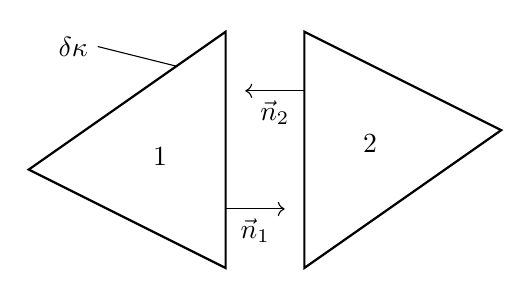
\begin{tikzpicture}

% Left triangle element "1"
\coordinate (A1) at ( 0.00,0.00);
\coordinate (A2) at ( 0.00,3.00);
\coordinate (A3) at (-2.50,1.25);
\node at (barycentric cs:A1=1,A2=1,A3=1) {1};
\draw[thick] (A1) -- (A2) -- (A3) -- cycle;
\draw[->] ($(A1)!0.25!(A2)$) -- +(0.75,0) node[midway,below] {$\vec{n}_1$};
\draw ($(A2)!0.25!(A3)$) -- +(-1.00,0.25) node[left] {$\delta \kappa$};

% Right triangle element "2"
\coordinate (B0) at ( 2.25,2.25); % center
\coordinate (B1) at ( 1.00,0.00);
\coordinate (B2) at ( 1.00,3.00);
\coordinate (B3) at ( 3.50,1.75);
\node at (barycentric cs:B1=1,B2=1,B3=1) {2};
\draw[thick] (B1) -- (B2) -- (B3) -- cycle;
\draw[->] ($(B1)!0.75!(B2)$) -- +(-0.75,0) node[midway,below] {$\vec{n}_2$};

\end{tikzpicture}

\end{document}
